\documentclass[1p]{elsarticle_modified}
%\bibliographystyle{elsarticle-num}

%\usepackage[colorlinks]{hyperref}
%\usepackage{abbrmath_seonhwa} %\Abb, \Ascr, \Acal ,\Abf, \Afrak
\usepackage{amsfonts}
\usepackage{amssymb}
\usepackage{amsmath}
\usepackage{amsthm}
\usepackage{scalefnt}
\usepackage{amsbsy}
\usepackage{kotex}
\usepackage{caption}
\usepackage{subfig}
\usepackage{color}
\usepackage{graphicx}
\usepackage{xcolor} %% white, black, red, green, blue, cyan, magenta, yellow
\usepackage{float}
\usepackage{setspace}
\usepackage{hyperref}

\usepackage{tikz}
\usetikzlibrary{arrows}

\usepackage{multirow}
\usepackage{array} % fixed length table
\usepackage{hhline}

%%%%%%%%%%%%%%%%%%%%%
\makeatletter
\renewcommand*\env@matrix[1][\arraystretch]{%
	\edef\arraystretch{#1}%
	\hskip -\arraycolsep
	\let\@ifnextchar\new@ifnextchar
	\array{*\c@MaxMatrixCols c}}
\makeatother %https://tex.stackexchange.com/questions/14071/how-can-i-increase-the-line-spacing-in-a-matrix
%%%%%%%%%%%%%%%

\usepackage[normalem]{ulem}

\newcommand{\msout}[1]{\ifmmode\text{\sout{\ensuremath{#1}}}\else\sout{#1}\fi}
%SOURCE: \msout is \stkout macro in https://tex.stackexchange.com/questions/20609/strikeout-in-math-mode

\newcommand{\cancel}[1]{
	\ifmmode
	{\color{red}\msout{#1}}
	\else
	{\color{red}\sout{#1}}
	\fi
}

\newcommand{\add}[1]{
	{\color{blue}\uwave{#1}}
}

\newcommand{\replace}[2]{
	\ifmmode
	{\color{red}\msout{#1}}{\color{blue}\uwave{#2}}
	\else
	{\color{red}\sout{#1}}{\color{blue}\uwave{#2}}
	\fi
}

\newcommand{\Sol}{\mathcal{S}} %segment
\newcommand{\D}{D} %diagram
\newcommand{\A}{\mathcal{A}} %arc


%%%%%%%%%%%%%%%%%%%%%%%%%%%%%5 test

\def\sl{\operatorname{\textup{SL}}(2,\Cbb)}
\def\psl{\operatorname{\textup{PSL}}(2,\Cbb)}
\def\quan{\mkern 1mu \triangleright \mkern 1mu}

\theoremstyle{definition}
\newtheorem{thm}{Theorem}[section]
\newtheorem{prop}[thm]{Proposition}
\newtheorem{lem}[thm]{Lemma}
\newtheorem{ques}[thm]{Question}
\newtheorem{cor}[thm]{Corollary}
\newtheorem{defn}[thm]{Definition}
\newtheorem{exam}[thm]{Example}
\newtheorem{rmk}[thm]{Remark}
\newtheorem{alg}[thm]{Algorithm}

\newcommand{\I}{\sqrt{-1}}
\begin{document}

%\begin{frontmatter}
%
%\title{Boundary parabolic representations of knots up to 8 crossings}
%
%%% Group authors per affiliation:
%\author{Yunhi Cho} 
%\address{Department of Mathematics, University of Seoul, Seoul, Korea}
%\ead{yhcho@uos.ac.kr}
%
%
%\author{Seonhwa Kim} %\fnref{s_kim}}
%\address{Center for Geometry and Physics, Institute for Basic Science, Pohang, 37673, Korea}
%\ead{ryeona17@ibs.re.kr}
%
%\author{Hyuk Kim}
%\address{Department of Mathematical Sciences, Seoul National University, Seoul 08826, Korea}
%\ead{hyukkim@snu.ac.kr}
%
%\author{Seokbeom Yoon}
%\address{Department of Mathematical Sciences, Seoul National University, Seoul, 08826,  Korea}
%\ead{sbyoon15@snu.ac.kr}
%
%\begin{abstract}
%We find all boundary parabolic representation of knots up to 8 crossings.
%
%\end{abstract}
%\begin{keyword}
%    \MSC[2010] 57M25 
%\end{keyword}
%
%\end{frontmatter}

%\linenumbers
%\tableofcontents
%
\newcommand\colored[1]{\textcolor{white}{\rule[-0.35ex]{0.8em}{1.4ex}}\kern-0.8em\color{red} #1}%
%\newcommand\colored[1]{\textcolor{white}{ #1}\kern-2.17ex	\textcolor{white}{ #1}\kern-1.81ex	\textcolor{white}{ #1}\kern-2.15ex\color{red}#1	}

{\Large $\underline{11a_{271}~(K11a_{271})}$}

\setlength{\tabcolsep}{10pt}
\renewcommand{\arraystretch}{1.6}
\vspace{1cm}\begin{tabular}{m{100pt}>{\centering\arraybackslash}m{274pt}}
\multirow{5}{120pt}{
	\centering
	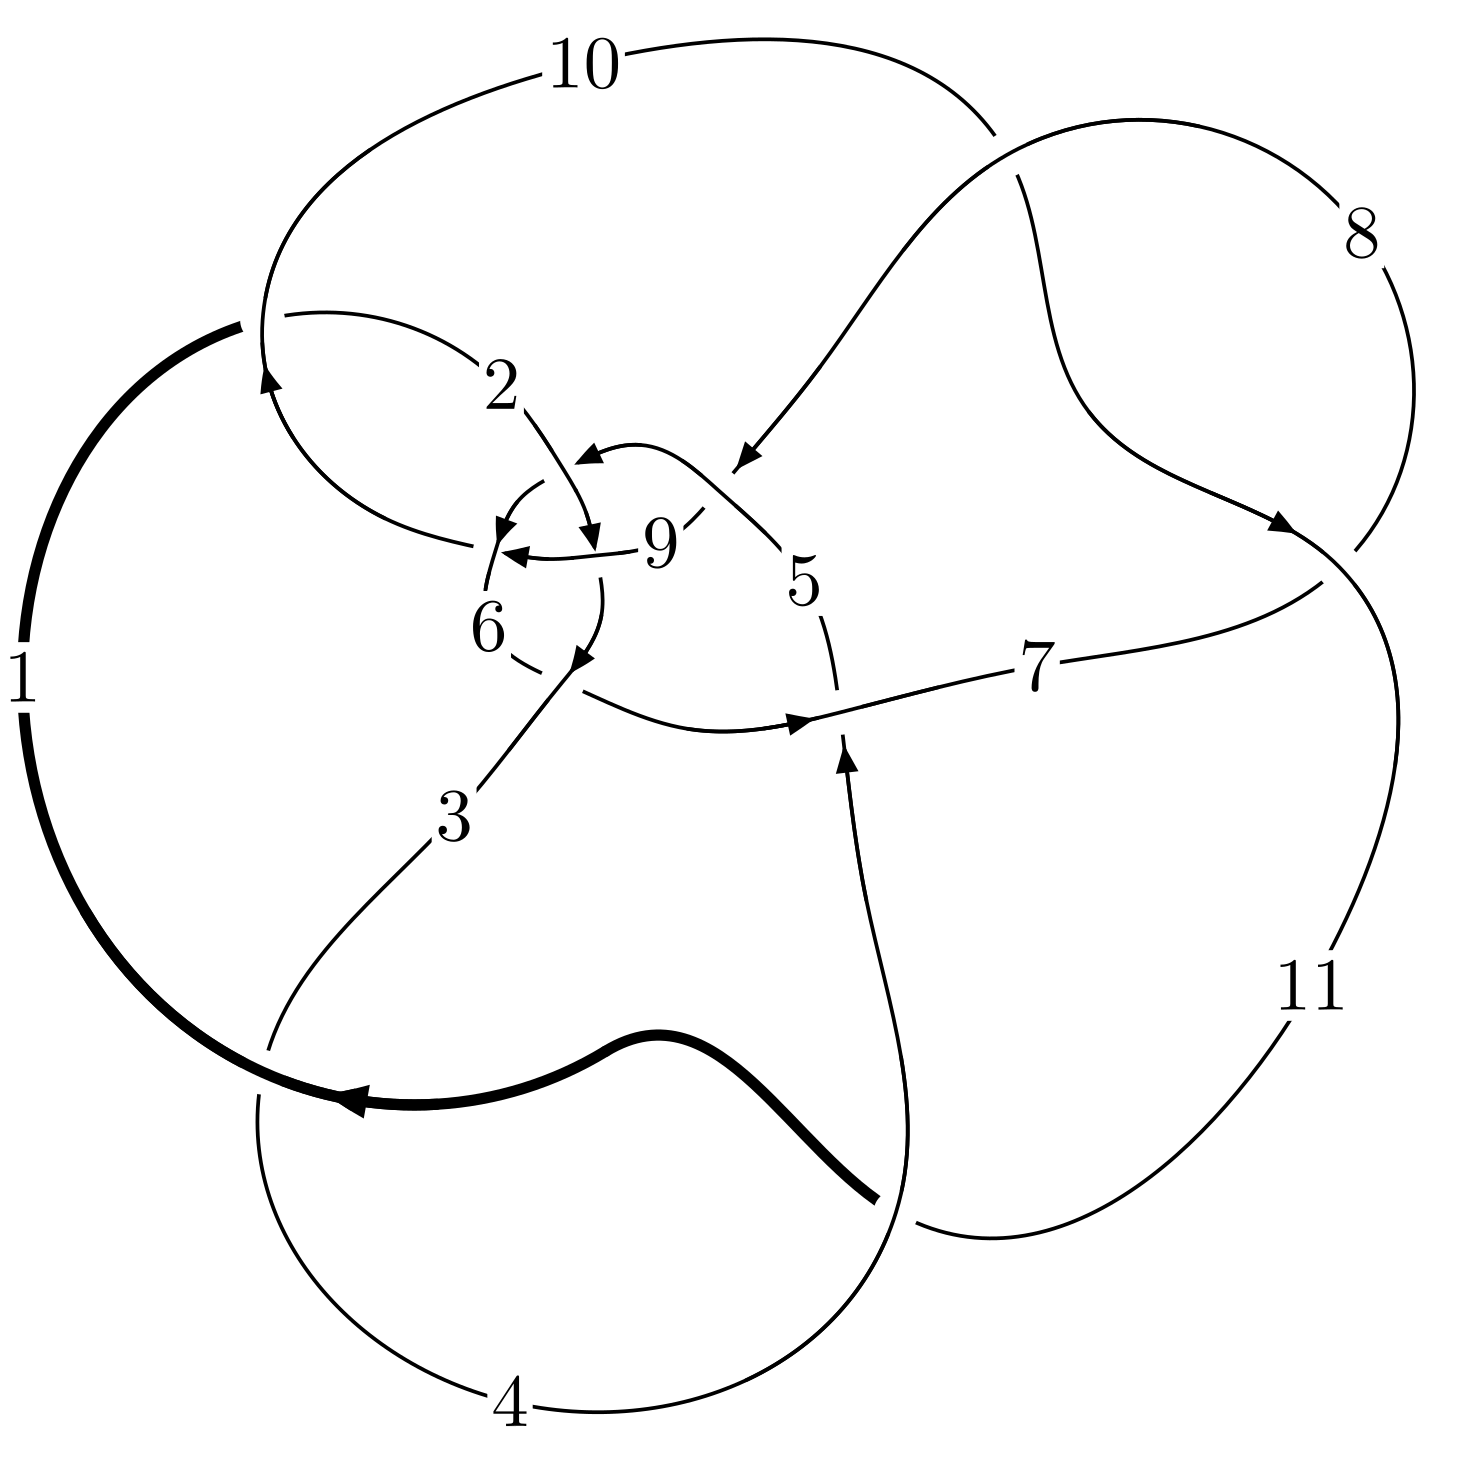
\includegraphics[width=112pt]{../../../GIT/diagram.site/Diagrams/png/520_11a_271.png}\\
\ \ \ A knot diagram\footnotemark}&
\allowdisplaybreaks
\textbf{Linearized knot diagam} \\
\cline{2-2}
 &
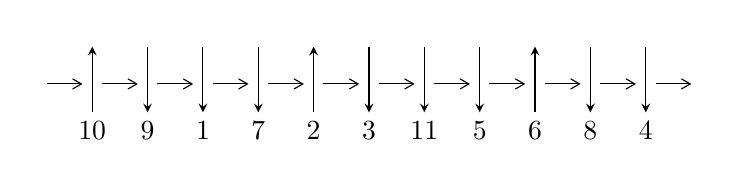
\begin{tikzpicture}[x=20pt, y=17pt]
	% nodes
	\node (C0) at (0, 0) {};
	\node (C1) at (1, 0) {};
	\node (C1U) at (1, +1) {};
	\node (C1D) at (1, -1) {10};

	\node (C2) at (2, 0) {};
	\node (C2U) at (2, +1) {};
	\node (C2D) at (2, -1) {9};

	\node (C3) at (3, 0) {};
	\node (C3U) at (3, +1) {};
	\node (C3D) at (3, -1) {1};

	\node (C4) at (4, 0) {};
	\node (C4U) at (4, +1) {};
	\node (C4D) at (4, -1) {7};

	\node (C5) at (5, 0) {};
	\node (C5U) at (5, +1) {};
	\node (C5D) at (5, -1) {2};

	\node (C6) at (6, 0) {};
	\node (C6U) at (6, +1) {};
	\node (C6D) at (6, -1) {3};

	\node (C7) at (7, 0) {};
	\node (C7U) at (7, +1) {};
	\node (C7D) at (7, -1) {11};

	\node (C8) at (8, 0) {};
	\node (C8U) at (8, +1) {};
	\node (C8D) at (8, -1) {5};

	\node (C9) at (9, 0) {};
	\node (C9U) at (9, +1) {};
	\node (C9D) at (9, -1) {6};

	\node (C10) at (10, 0) {};
	\node (C10U) at (10, +1) {};
	\node (C10D) at (10, -1) {8};

	\node (C11) at (11, 0) {};
	\node (C11U) at (11, +1) {};
	\node (C11D) at (11, -1) {4};
	\node (C12) at (12, 0) {};

	% arrows
	\draw[->,>={angle 60}]
	(C0) edge (C1) (C1) edge (C2) (C2) edge (C3) (C3) edge (C4) (C4) edge (C5) (C5) edge (C6) (C6) edge (C7) (C7) edge (C8) (C8) edge (C9) (C9) edge (C10) (C10) edge (C11) (C11) edge (C12) ;	\draw[->,>=stealth]
	(C1D) edge (C1U) (C2U) edge (C2D) (C3U) edge (C3D) (C4U) edge (C4D) (C5D) edge (C5U) (C6U) edge (C6D) (C7U) edge (C7D) (C8U) edge (C8D) (C9D) edge (C9U) (C10U) edge (C10D) (C11U) edge (C11D) ;
	\end{tikzpicture} \\
\hhline{~~} \\& 
\textbf{Solving Sequence} \\ \cline{2-2} 
 &
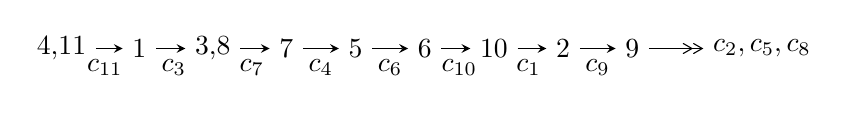
\begin{tikzpicture}[x=25pt, y=7pt]
	% node
	\node (A0) at (-1/8, 0) {4,11};
	\node (A1) at (1, 0) {1};
	\node (A2) at (33/16, 0) {3,8};
	\node (A3) at (25/8, 0) {7};
	\node (A4) at (33/8, 0) {5};
	\node (A5) at (41/8, 0) {6};
	\node (A6) at (49/8, 0) {10};
	\node (A7) at (57/8, 0) {2};
	\node (A8) at (65/8, 0) {9};
	\node (C1) at (1/2, -1) {$c_{11}$};
	\node (C2) at (3/2, -1) {$c_{3}$};
	\node (C3) at (21/8, -1) {$c_{7}$};
	\node (C4) at (29/8, -1) {$c_{4}$};
	\node (C5) at (37/8, -1) {$c_{6}$};
	\node (C6) at (45/8, -1) {$c_{10}$};
	\node (C7) at (53/8, -1) {$c_{1}$};
	\node (C8) at (61/8, -1) {$c_{9}$};
	\node (A9) at (10, 0) {$c_{2},c_{5},c_{8}$};

	% edge
	\draw[->,>=stealth]	
	(A0) edge (A1) (A1) edge (A2) (A2) edge (A3) (A3) edge (A4) (A4) edge (A5) (A5) edge (A6) (A6) edge (A7) (A7) edge (A8) ;
	\draw[->>,>={angle 60}]	
	(A8) edge (A9);
\end{tikzpicture} \\ 

\end{tabular} \\

\footnotetext{
The image of knot diagram is generated by the software ``\textbf{Draw programme}" developed by Andrew Bartholomew(\url{http://www.layer8.co.uk/maths/draw/index.htm\#Running-draw}), where we modified some parts for our purpose(\url{https://github.com/CATsTAILs/LinksPainter}).
}\phantom \\ \newline 
\centering \textbf{Ideals for irreducible components\footnotemark of $X_{\text{par}}$} 
 
\begin{align*}
I^u_{1}&=\langle 
b- u,\;-1787419727 u^{22}+404361799 u^{21}+\cdots+1141379489 a-6968741388,\\
\phantom{I^u_{1}}&\phantom{= \langle  }u^{23}+10 u^{21}+\cdots+6 u+1\rangle \\
I^u_{2}&=\langle 
-8.66938\times10^{235} u^{81}-4.61286\times10^{236} u^{80}+\cdots+7.40850\times10^{236} b-6.46383\times10^{238},\\
\phantom{I^u_{2}}&\phantom{= \langle  }4.79729\times10^{238} u^{81}+3.73078\times10^{239} u^{80}+\cdots+4.31916\times10^{239} a+1.02668\times10^{242},\\
\phantom{I^u_{2}}&\phantom{= \langle  }u^{82}+4 u^{81}+\cdots+1581 u+583\rangle \\
I^u_{3}&=\langle 
b+u,\;-2 u^7+u^6-6 u^5+u^4-6 u^3+a,\;u^8- u^7+4 u^6-3 u^5+6 u^4-4 u^3+3 u^2-2 u+1\rangle \\
I^u_{4}&=\langle 
12 u^9-27 u^8+100 u^7-154 u^6+247 u^5-252 u^4+225 u^3-149 u^2+b+59 u-16,\\
\phantom{I^u_{4}}&\phantom{= \langle  }- u^9+3 u^8-11 u^7+21 u^6-37 u^5+45 u^4-46 u^3+34 u^2+a-18 u+6,\\
\phantom{I^u_{4}}&\phantom{= \langle  }u^{10}-3 u^9+10 u^8-19 u^7+30 u^6-36 u^5+34 u^4-26 u^3+14 u^2-5 u+1\rangle \\
I^u_{5}&=\langle 
b+u,\;a- u+1,\;u^2- u+1\rangle \\
\\
\end{align*}
\raggedright * 5 irreducible components of $\dim_{\mathbb{C}}=0$, with total 125 representations.\\
\footnotetext{All coefficients of polynomials are rational numbers. But the coefficients are sometimes approximated in decimal forms when there is not enough margin.}
\newpage
\renewcommand{\arraystretch}{1}
\centering \section*{I. $I^u_{1}= \langle b- u,\;-1.79\times10^{9} u^{22}+4.04\times10^{8} u^{21}+\cdots+1.14\times10^{9} a-6.97\times10^{9},\;u^{23}+10 u^{21}+\cdots+6 u+1 \rangle$}
\flushleft \textbf{(i) Arc colorings}\\
\begin{tabular}{m{7pt} m{180pt} m{7pt} m{180pt} }
\flushright $a_{4}=$&$\begin{pmatrix}0\\u\end{pmatrix}$ \\
\flushright $a_{11}=$&$\begin{pmatrix}1\\0\end{pmatrix}$ \\
\flushright $a_{1}=$&$\begin{pmatrix}1\\u^2\end{pmatrix}$ \\
\flushright $a_{3}=$&$\begin{pmatrix}u\\u^3+u\end{pmatrix}$ \\
\flushright $a_{8}=$&$\begin{pmatrix}1.56602 u^{22}-0.354275 u^{21}+\cdots+5.26162 u+6.10554\\u\end{pmatrix}$ \\
\flushright $a_{7}=$&$\begin{pmatrix}1.56602 u^{22}-0.354275 u^{21}+\cdots+6.26162 u+6.10554\\u\end{pmatrix}$ \\
\flushright $a_{5}=$&$\begin{pmatrix}-0.0100717 u^{22}-0.0618659 u^{21}+\cdots+9.45541 u+7.55747\\0.474519 u^{22}+0.0483773 u^{21}+\cdots+0.440369 u-0.354275\end{pmatrix}$ \\
\flushright $a_{6}=$&$\begin{pmatrix}1.43020 u^{22}-0.552730 u^{21}+\cdots+4.93721 u+5.70289\\-0.0398045 u^{22}+0.0200600 u^{21}+\cdots+1.00214 u-0.204197\end{pmatrix}$ \\
\flushright $a_{10}=$&$\begin{pmatrix}0.354275 u^{22}+0.474519 u^{21}+\cdots+3.29056 u+2.56602\\- u^2\end{pmatrix}$ \\
\flushright $a_{2}=$&$\begin{pmatrix}-0.515155 u^{22}+1.53719 u^{21}+\cdots+7.98960 u+2.53517\\0.246833 u^{22}-0.706353 u^{21}+\cdots-3.61365 u-0.610339\end{pmatrix}$ \\
\flushright $a_{9}=$&$\begin{pmatrix}-1.76578 u^{22}+0.872515 u^{21}+\cdots+0.752076 u-1.55408\\0.528715 u^{22}-0.182288 u^{21}+\cdots+0.732677 u+0.346273\end{pmatrix}$\\ \flushright $a_{9}=$&$\begin{pmatrix}-1.76578 u^{22}+0.872515 u^{21}+\cdots+0.752076 u-1.55408\\0.528715 u^{22}-0.182288 u^{21}+\cdots+0.732677 u+0.346273\end{pmatrix}$\\&\end{tabular}
\flushleft \textbf{(ii) Obstruction class $= -1$}\\~\\
\flushleft \textbf{(iii) Cusp Shapes $= \frac{1113912392}{1141379489} u^{22}+\frac{1733888615}{1141379489} u^{21}+\cdots+\frac{15405030005}{1141379489} u+\frac{4456929967}{1141379489}$}\\~\\
\newpage\renewcommand{\arraystretch}{1}
\flushleft \textbf{(iv) u-Polynomials at the component}\newline \\
\begin{tabular}{m{50pt}|m{274pt}}
Crossings & \hspace{64pt}u-Polynomials at each crossing \\
\hline $$\begin{aligned}c_{1}\end{aligned}$$&$\begin{aligned}
&u^{23}+22 u^{22}+\cdots+7424 u+512
\end{aligned}$\\
\hline $$\begin{aligned}c_{2}\end{aligned}$$&$\begin{aligned}
&u^{23}+19 u^{22}+\cdots-96 u-16
\end{aligned}$\\
\hline $$\begin{aligned}c_{3},c_{7},c_{10}\\c_{11}\end{aligned}$$&$\begin{aligned}
&u^{23}+10 u^{21}+\cdots+6 u+1
\end{aligned}$\\
\hline $$\begin{aligned}c_{4}\end{aligned}$$&$\begin{aligned}
&u^{23}-19 u^{22}+\cdots-960 u+256
\end{aligned}$\\
\hline $$\begin{aligned}c_{5},c_{9}\end{aligned}$$&$\begin{aligned}
&u^{23}- u^{22}+\cdots- u+1
\end{aligned}$\\
\hline $$\begin{aligned}c_{6},c_{8}\end{aligned}$$&$\begin{aligned}
&u^{23}- u^{22}+\cdots+4 u+4
\end{aligned}$\\
\hline
\end{tabular}\\~\\
\newpage\renewcommand{\arraystretch}{1}
\flushleft \textbf{(v) Riley Polynomials at the component}\newline \\
\begin{tabular}{m{50pt}|m{274pt}}
Crossings & \hspace{64pt}Riley Polynomials at each crossing \\
\hline $$\begin{aligned}c_{1}\end{aligned}$$&$\begin{aligned}
&y^{23}-2 y^{22}+\cdots+11599872 y-262144
\end{aligned}$\\
\hline $$\begin{aligned}c_{2}\end{aligned}$$&$\begin{aligned}
&y^{23}-5 y^{22}+\cdots-6016 y-256
\end{aligned}$\\
\hline $$\begin{aligned}c_{3},c_{7},c_{10}\\c_{11}\end{aligned}$$&$\begin{aligned}
&y^{23}+20 y^{22}+\cdots+20 y-1
\end{aligned}$\\
\hline $$\begin{aligned}c_{4}\end{aligned}$$&$\begin{aligned}
&y^{23}-7 y^{22}+\cdots+1011712 y-65536
\end{aligned}$\\
\hline $$\begin{aligned}c_{5},c_{9}\end{aligned}$$&$\begin{aligned}
&y^{23}-3 y^{22}+\cdots-3 y-1
\end{aligned}$\\
\hline $$\begin{aligned}c_{6},c_{8}\end{aligned}$$&$\begin{aligned}
&y^{23}-9 y^{22}+\cdots+80 y-16
\end{aligned}$\\
\hline
\end{tabular}\\~\\
\newpage\flushleft \textbf{(vi) Complex Volumes and Cusp Shapes}
$$\begin{array}{c|c|c}  
\text{Solutions to }I^u_{1}& \I (\text{vol} + \sqrt{-1}CS) & \text{Cusp shape}\\
 \hline 
\begin{aligned}
u &= \phantom{-}0.097203 + 1.048750 I \\
a &= -0.88581 - 3.73190 I \\
b &= \phantom{-}0.097203 + 1.048750 I\end{aligned}
 & \phantom{-}0.41923 - 7.68149 I & -2.73500 + 7.62634 I \\ \hline\begin{aligned}
u &= \phantom{-}0.097203 - 1.048750 I \\
a &= -0.88581 + 3.73190 I \\
b &= \phantom{-}0.097203 - 1.048750 I\end{aligned}
 & \phantom{-}0.41923 + 7.68149 I & -2.73500 - 7.62634 I \\ \hline\begin{aligned}
u &= -0.878283 + 0.234924 I \\
a &= -0.069448 - 0.504553 I \\
b &= -0.878283 + 0.234924 I\end{aligned}
 & -4.00620 + 1.06800 I & -20.0904 - 5.7474 I \\ \hline\begin{aligned}
u &= -0.878283 - 0.234924 I \\
a &= -0.069448 + 0.504553 I \\
b &= -0.878283 - 0.234924 I\end{aligned}
 & -4.00620 - 1.06800 I & -20.0904 + 5.7474 I \\ \hline\begin{aligned}
u &= \phantom{-}0.832612 + 0.199739 I \\
a &= \phantom{-}0.269970 - 0.994841 I \\
b &= \phantom{-}0.832612 + 0.199739 I\end{aligned}
 & -4.74103 + 7.77621 I & -9.99957 - 4.77400 I \\ \hline\begin{aligned}
u &= \phantom{-}0.832612 - 0.199739 I \\
a &= \phantom{-}0.269970 + 0.994841 I \\
b &= \phantom{-}0.832612 - 0.199739 I\end{aligned}
 & -4.74103 - 7.77621 I & -9.99957 + 4.77400 I \\ \hline\begin{aligned}
u &= \phantom{-}0.086667 + 1.177120 I \\
a &= \phantom{-}0.91809 - 1.64121 I \\
b &= \phantom{-}0.086667 + 1.177120 I\end{aligned}
 & \phantom{-}4.82355 + 1.72572 I & \phantom{-}1.86379 - 3.16589 I \\ \hline\begin{aligned}
u &= \phantom{-}0.086667 - 1.177120 I \\
a &= \phantom{-}0.91809 + 1.64121 I \\
b &= \phantom{-}0.086667 - 1.177120 I\end{aligned}
 & \phantom{-}4.82355 - 1.72572 I & \phantom{-}1.86379 + 3.16589 I \\ \hline\begin{aligned}
u &= \phantom{-}0.485747 + 0.587883 I \\
a &= \phantom{-}0.867752 + 0.473235 I \\
b &= \phantom{-}0.485747 + 0.587883 I\end{aligned}
 & -1.41194 + 2.54862 I & -8.72632 - 1.31178 I \\ \hline\begin{aligned}
u &= \phantom{-}0.485747 - 0.587883 I \\
a &= \phantom{-}0.867752 - 0.473235 I \\
b &= \phantom{-}0.485747 - 0.587883 I\end{aligned}
 & -1.41194 - 2.54862 I & -8.72632 + 1.31178 I\\
 \hline 
 \end{array}$$\newpage$$\begin{array}{c|c|c}  
\text{Solutions to }I^u_{1}& \I (\text{vol} + \sqrt{-1}CS) & \text{Cusp shape}\\
 \hline 
\begin{aligned}
u &= -0.332148 + 1.312160 I \\
a &= -1.15057 - 2.08899 I \\
b &= -0.332148 + 1.312160 I\end{aligned}
 & \phantom{-}6.09809 + 8.12392 I & \phantom{-}3.40597 - 8.83423 I \\ \hline\begin{aligned}
u &= -0.332148 - 1.312160 I \\
a &= -1.15057 + 2.08899 I \\
b &= -0.332148 - 1.312160 I\end{aligned}
 & \phantom{-}6.09809 - 8.12392 I & \phantom{-}3.40597 + 8.83423 I \\ \hline\begin{aligned}
u &= \phantom{-}0.33824 + 1.37393 I \\
a &= \phantom{-}0.69111 - 1.66289 I \\
b &= \phantom{-}0.33824 + 1.37393 I\end{aligned}
 & \phantom{-}9.61085 - 2.02294 I & \phantom{-}3.47785 + 0.15643 I \\ \hline\begin{aligned}
u &= \phantom{-}0.33824 - 1.37393 I \\
a &= \phantom{-}0.69111 + 1.66289 I \\
b &= \phantom{-}0.33824 - 1.37393 I\end{aligned}
 & \phantom{-}9.61085 + 2.02294 I & \phantom{-}3.47785 - 0.15643 I \\ \hline\begin{aligned}
u &= -0.25671 + 1.41656 I \\
a &= -0.16528 - 1.74879 I \\
b &= -0.25671 + 1.41656 I\end{aligned}
 & \phantom{-}6.46756 + 3.72990 I & \phantom{-}2.37255 - 3.19850 I \\ \hline\begin{aligned}
u &= -0.25671 - 1.41656 I \\
a &= -0.16528 + 1.74879 I \\
b &= -0.25671 - 1.41656 I\end{aligned}
 & \phantom{-}6.46756 - 3.72990 I & \phantom{-}2.37255 + 3.19850 I \\ \hline\begin{aligned}
u &= -0.50959 + 1.43123 I \\
a &= -0.44449 - 1.89615 I \\
b &= -0.50959 + 1.43123 I\end{aligned}
 & \phantom{-}3.75645 + 9.55892 I & -6.8688 - 15.7902 I \\ \hline\begin{aligned}
u &= -0.50959 - 1.43123 I \\
a &= -0.44449 + 1.89615 I \\
b &= -0.50959 - 1.43123 I\end{aligned}
 & \phantom{-}3.75645 - 9.55892 I & -6.8688 + 15.7902 I \\ \hline\begin{aligned}
u &= \phantom{-}0.56914 + 1.42280 I \\
a &= \phantom{-}0.59171 - 1.70238 I \\
b &= \phantom{-}0.56914 + 1.42280 I\end{aligned}
 & \phantom{-}3.0635 - 18.7890 I & -2.94689 + 9.73353 I \\ \hline\begin{aligned}
u &= \phantom{-}0.56914 - 1.42280 I \\
a &= \phantom{-}0.59171 + 1.70238 I \\
b &= \phantom{-}0.56914 - 1.42280 I\end{aligned}
 & \phantom{-}3.0635 + 18.7890 I & -2.94689 - 9.73353 I\\
 \hline 
 \end{array}$$\newpage$$\begin{array}{c|c|c}  
\text{Solutions to }I^u_{1}& \I (\text{vol} + \sqrt{-1}CS) & \text{Cusp shape}\\
 \hline 
\begin{aligned}
u &= -0.329226 + 0.326454 I \\
a &= \phantom{-}1.012200 + 0.058405 I \\
b &= -0.329226 + 0.326454 I\end{aligned}
 & -0.744276 + 1.012620 I & -5.79242 - 5.25340 I \\ \hline\begin{aligned}
u &= -0.329226 - 0.326454 I \\
a &= \phantom{-}1.012200 - 0.058405 I \\
b &= -0.329226 - 0.326454 I\end{aligned}
 & -0.744276 - 1.012620 I & -5.79242 + 5.25340 I \\ \hline\begin{aligned}
u &= -0.207295\phantom{ +0.000000I} \\
a &= \phantom{-}5.72955\phantom{ +0.000000I} \\
b &= -0.207295\phantom{ +0.000000I}\end{aligned}
 & -2.25842\phantom{ +0.000000I} & \phantom{-}3.07840\phantom{ +0.000000I}\\
 \hline 
 \end{array}$$\newpage\newpage\renewcommand{\arraystretch}{1}
\centering \section*{II. $I^u_{2}= \langle -8.67\times10^{235} u^{81}-4.61\times10^{236} u^{80}+\cdots+7.41\times10^{236} b-6.46\times10^{238},\;4.80\times10^{238} u^{81}+3.73\times10^{239} u^{80}+\cdots+4.32\times10^{239} a+1.03\times10^{242},\;u^{82}+4 u^{81}+\cdots+1581 u+583 \rangle$}
\flushleft \textbf{(i) Arc colorings}\\
\begin{tabular}{m{7pt} m{180pt} m{7pt} m{180pt} }
\flushright $a_{4}=$&$\begin{pmatrix}0\\u\end{pmatrix}$ \\
\flushright $a_{11}=$&$\begin{pmatrix}1\\0\end{pmatrix}$ \\
\flushright $a_{1}=$&$\begin{pmatrix}1\\u^2\end{pmatrix}$ \\
\flushright $a_{3}=$&$\begin{pmatrix}u\\u^3+u\end{pmatrix}$ \\
\flushright $a_{8}=$&$\begin{pmatrix}-0.111070 u^{81}-0.863775 u^{80}+\cdots-708.703 u-237.704\\0.117019 u^{81}+0.622644 u^{80}+\cdots+301.616 u+87.2488\end{pmatrix}$ \\
\flushright $a_{7}=$&$\begin{pmatrix}0.00594924 u^{81}-0.241131 u^{80}+\cdots-407.086 u-150.455\\0.117019 u^{81}+0.622644 u^{80}+\cdots+301.616 u+87.2488\end{pmatrix}$ \\
\flushright $a_{5}=$&$\begin{pmatrix}-0.219221 u^{81}-1.23505 u^{80}+\cdots-634.131 u-201.913\\0.150861 u^{81}+0.982201 u^{80}+\cdots+631.616 u+195.251\end{pmatrix}$ \\
\flushright $a_{6}=$&$\begin{pmatrix}-0.133406 u^{81}-0.938320 u^{80}+\cdots-706.882 u-233.890\\0.131216 u^{81}+0.674433 u^{80}+\cdots+304.040 u+85.3005\end{pmatrix}$ \\
\flushright $a_{10}=$&$\begin{pmatrix}-0.344459 u^{81}-1.29164 u^{80}+\cdots-52.0179 u+50.8287\\0.00955082 u^{81}+0.102874 u^{80}+\cdots+152.659 u+51.2985\end{pmatrix}$ \\
\flushright $a_{2}=$&$\begin{pmatrix}-0.605273 u^{81}-2.16854 u^{80}+\cdots+61.9906 u+135.141\\0.382816 u^{81}+1.45114 u^{80}+\cdots+16.4038 u-62.7682\end{pmatrix}$ \\
\flushright $a_{9}=$&$\begin{pmatrix}-0.344825 u^{81}-1.48129 u^{80}+\cdots-184.980 u-9.26806\\0.138777 u^{81}+0.708851 u^{80}+\cdots+267.957 u+70.7972\end{pmatrix}$\\ \flushright $a_{9}=$&$\begin{pmatrix}-0.344825 u^{81}-1.48129 u^{80}+\cdots-184.980 u-9.26806\\0.138777 u^{81}+0.708851 u^{80}+\cdots+267.957 u+70.7972\end{pmatrix}$\\&\end{tabular}
\flushleft \textbf{(ii) Obstruction class $= -1$}\\~\\
\flushleft \textbf{(iii) Cusp Shapes $= 0.557208 u^{81}+1.61916 u^{80}+\cdots-644.455 u-351.850$}\\~\\
\newpage\renewcommand{\arraystretch}{1}
\flushleft \textbf{(iv) u-Polynomials at the component}\newline \\
\begin{tabular}{m{50pt}|m{274pt}}
Crossings & \hspace{64pt}u-Polynomials at each crossing \\
\hline $$\begin{aligned}c_{1}\end{aligned}$$&$\begin{aligned}
&(u^{41}-7 u^{40}+\cdots-13 u+1)^{2}
\end{aligned}$\\
\hline $$\begin{aligned}c_{2}\end{aligned}$$&$\begin{aligned}
&(u^{41}-8 u^{40}+\cdots+2 u-1)^{2}
\end{aligned}$\\
\hline $$\begin{aligned}c_{3},c_{7},c_{10}\\c_{11}\end{aligned}$$&$\begin{aligned}
&u^{82}+4 u^{81}+\cdots+1581 u+583
\end{aligned}$\\
\hline $$\begin{aligned}c_{4}\end{aligned}$$&$\begin{aligned}
&(u^{41}+11 u^{40}+\cdots+92 u+11)^{2}
\end{aligned}$\\
\hline $$\begin{aligned}c_{5},c_{9}\end{aligned}$$&$\begin{aligned}
&u^{82}-5 u^{81}+\cdots+61 u+11
\end{aligned}$\\
\hline $$\begin{aligned}c_{6},c_{8}\end{aligned}$$&$\begin{aligned}
&u^{82}+u^{81}+\cdots-5311 u+961
\end{aligned}$\\
\hline
\end{tabular}\\~\\
\newpage\renewcommand{\arraystretch}{1}
\flushleft \textbf{(v) Riley Polynomials at the component}\newline \\
\begin{tabular}{m{50pt}|m{274pt}}
Crossings & \hspace{64pt}Riley Polynomials at each crossing \\
\hline $$\begin{aligned}c_{1}\end{aligned}$$&$\begin{aligned}
&(y^{41}+11 y^{40}+\cdots+9 y-1)^{2}
\end{aligned}$\\
\hline $$\begin{aligned}c_{2}\end{aligned}$$&$\begin{aligned}
&(y^{41}-8 y^{40}+\cdots+30 y-1)^{2}
\end{aligned}$\\
\hline $$\begin{aligned}c_{3},c_{7},c_{10}\\c_{11}\end{aligned}$$&$\begin{aligned}
&y^{82}+58 y^{81}+\cdots+8444515 y+339889
\end{aligned}$\\
\hline $$\begin{aligned}c_{4}\end{aligned}$$&$\begin{aligned}
&(y^{41}+13 y^{40}+\cdots-1898 y-121)^{2}
\end{aligned}$\\
\hline $$\begin{aligned}c_{5},c_{9}\end{aligned}$$&$\begin{aligned}
&y^{82}+13 y^{81}+\cdots+6949 y+121
\end{aligned}$\\
\hline $$\begin{aligned}c_{6},c_{8}\end{aligned}$$&$\begin{aligned}
&y^{82}-31 y^{81}+\cdots-8782989 y+923521
\end{aligned}$\\
\hline
\end{tabular}\\~\\
\newpage\flushleft \textbf{(vi) Complex Volumes and Cusp Shapes}
$$\begin{array}{c|c|c}  
\text{Solutions to }I^u_{2}& \I (\text{vol} + \sqrt{-1}CS) & \text{Cusp shape}\\
 \hline 
\begin{aligned}
u &= -0.201433 + 0.974457 I \\
a &= -0.24847 - 2.21630 I \\
b &= -0.50859 + 1.75201 I\end{aligned}
 & \phantom{-}2.07268 + 5.10749 I & \phantom{-0.000000 } 0 \\ \hline\begin{aligned}
u &= -0.201433 - 0.974457 I \\
a &= -0.24847 + 2.21630 I \\
b &= -0.50859 - 1.75201 I\end{aligned}
 & \phantom{-}2.07268 - 5.10749 I & \phantom{-0.000000 } 0 \\ \hline\begin{aligned}
u &= -0.766022 + 0.674504 I \\
a &= \phantom{-}0.802065 + 0.258031 I \\
b &= \phantom{-}0.411623 - 1.052910 I\end{aligned}
 & \phantom{-}0.21627 + 5.92950 I & \phantom{-0.000000 } 0 \\ \hline\begin{aligned}
u &= -0.766022 - 0.674504 I \\
a &= \phantom{-}0.802065 - 0.258031 I \\
b &= \phantom{-}0.411623 + 1.052910 I\end{aligned}
 & \phantom{-}0.21627 - 5.92950 I & \phantom{-0.000000 } 0 \\ \hline\begin{aligned}
u &= \phantom{-}0.046473 + 1.022060 I \\
a &= \phantom{-}0.0453885 - 0.0654803 I \\
b &= -0.908235 + 0.579105 I\end{aligned}
 & -0.195730 - 0.062095 I & \phantom{-0.000000 } 0 \\ \hline\begin{aligned}
u &= \phantom{-}0.046473 - 1.022060 I \\
a &= \phantom{-}0.0453885 + 0.0654803 I \\
b &= -0.908235 - 0.579105 I\end{aligned}
 & -0.195730 + 0.062095 I & \phantom{-0.000000 } 0 \\ \hline\begin{aligned}
u &= \phantom{-}0.481687 + 0.914453 I \\
a &= -0.952194 - 0.769085 I \\
b &= \phantom{-}0.104564 - 0.731487 I\end{aligned}
 & -0.53309 - 6.66067 I & \phantom{-0.000000 } 0 \\ \hline\begin{aligned}
u &= \phantom{-}0.481687 - 0.914453 I \\
a &= -0.952194 + 0.769085 I \\
b &= \phantom{-}0.104564 + 0.731487 I\end{aligned}
 & -0.53309 + 6.66067 I & \phantom{-0.000000 } 0 \\ \hline\begin{aligned}
u &= -0.084502 + 0.953123 I \\
a &= \phantom{-}0.27716 + 3.12610 I \\
b &= -0.084502 - 0.953123 I\end{aligned}
 & -1.00058\phantom{ +0.000000I} & \phantom{-0.000000 } 0 \\ \hline\begin{aligned}
u &= -0.084502 - 0.953123 I \\
a &= \phantom{-}0.27716 - 3.12610 I \\
b &= -0.084502 + 0.953123 I\end{aligned}
 & -1.00058\phantom{ +0.000000I} & \phantom{-0.000000 } 0\\
 \hline 
 \end{array}$$\newpage$$\begin{array}{c|c|c}  
\text{Solutions to }I^u_{2}& \I (\text{vol} + \sqrt{-1}CS) & \text{Cusp shape}\\
 \hline 
\begin{aligned}
u &= \phantom{-}0.908053 + 0.267502 I \\
a &= \phantom{-}0.122614 - 0.116976 I \\
b &= -0.436052 + 1.232410 I\end{aligned}
 & \phantom{-}0.05211 + 4.45406 I & \phantom{-0.000000 } 0 \\ \hline\begin{aligned}
u &= \phantom{-}0.908053 - 0.267502 I \\
a &= \phantom{-}0.122614 + 0.116976 I \\
b &= -0.436052 - 1.232410 I\end{aligned}
 & \phantom{-}0.05211 - 4.45406 I & \phantom{-0.000000 } 0 \\ \hline\begin{aligned}
u &= \phantom{-}0.356623 + 0.993352 I \\
a &= \phantom{-}0.318656 + 0.614201 I \\
b &= -1.239790 - 0.228596 I\end{aligned}
 & -1.92162 - 3.53381 I & \phantom{-0.000000 } 0 \\ \hline\begin{aligned}
u &= \phantom{-}0.356623 - 0.993352 I \\
a &= \phantom{-}0.318656 - 0.614201 I \\
b &= -1.239790 + 0.228596 I\end{aligned}
 & -1.92162 + 3.53381 I & \phantom{-0.000000 } 0 \\ \hline\begin{aligned}
u &= -0.908235 + 0.579105 I \\
a &= -0.0324041 - 0.0683877 I \\
b &= \phantom{-}0.046473 + 1.022060 I\end{aligned}
 & -0.195730 - 0.062095 I & \phantom{-0.000000 } 0 \\ \hline\begin{aligned}
u &= -0.908235 - 0.579105 I \\
a &= -0.0324041 + 0.0683877 I \\
b &= \phantom{-}0.046473 - 1.022060 I\end{aligned}
 & -0.195730 + 0.062095 I & \phantom{-0.000000 } 0 \\ \hline\begin{aligned}
u &= \phantom{-}0.068284 + 1.081370 I \\
a &= -0.96185 + 2.05879 I \\
b &= -0.42203 - 1.39285 I\end{aligned}
 & \phantom{-}5.03352 - 3.32205 I & \phantom{-0.000000 } 0 \\ \hline\begin{aligned}
u &= \phantom{-}0.068284 - 1.081370 I \\
a &= -0.96185 - 2.05879 I \\
b &= -0.42203 + 1.39285 I\end{aligned}
 & \phantom{-}5.03352 + 3.32205 I & \phantom{-0.000000 } 0 \\ \hline\begin{aligned}
u &= -0.333019 + 1.053950 I \\
a &= \phantom{-}0.318558 + 0.572725 I \\
b &= -0.818658 - 0.168076 I\end{aligned}
 & \phantom{-}0.116913 + 1.387900 I & \phantom{-0.000000 } 0 \\ \hline\begin{aligned}
u &= -0.333019 - 1.053950 I \\
a &= \phantom{-}0.318558 - 0.572725 I \\
b &= -0.818658 + 0.168076 I\end{aligned}
 & \phantom{-}0.116913 - 1.387900 I & \phantom{-0.000000 } 0\\
 \hline 
 \end{array}$$\newpage$$\begin{array}{c|c|c}  
\text{Solutions to }I^u_{2}& \I (\text{vol} + \sqrt{-1}CS) & \text{Cusp shape}\\
 \hline 
\begin{aligned}
u &= \phantom{-}0.044484 + 1.105450 I \\
a &= -0.10256 + 2.32484 I \\
b &= \phantom{-}0.46839 - 1.96413 I\end{aligned}
 & \phantom{-}3.54374 - 4.65960 I & \phantom{-0.000000 } 0 \\ \hline\begin{aligned}
u &= \phantom{-}0.044484 - 1.105450 I \\
a &= -0.10256 - 2.32484 I \\
b &= \phantom{-}0.46839 + 1.96413 I\end{aligned}
 & \phantom{-}3.54374 + 4.65960 I & \phantom{-0.000000 } 0 \\ \hline\begin{aligned}
u &= \phantom{-}0.133627 + 1.121670 I \\
a &= -0.10313 + 2.45385 I \\
b &= -0.49419 - 1.57359 I\end{aligned}
 & \phantom{-}2.42232 - 4.46231 I & \phantom{-0.000000 } 0 \\ \hline\begin{aligned}
u &= \phantom{-}0.133627 - 1.121670 I \\
a &= -0.10313 - 2.45385 I \\
b &= -0.49419 + 1.57359 I\end{aligned}
 & \phantom{-}2.42232 + 4.46231 I & \phantom{-0.000000 } 0 \\ \hline\begin{aligned}
u &= \phantom{-}0.411623 + 1.052910 I \\
a &= -0.536788 + 0.538970 I \\
b &= -0.766022 - 0.674504 I\end{aligned}
 & \phantom{-}0.21627 - 5.92950 I & \phantom{-0.000000 } 0 \\ \hline\begin{aligned}
u &= \phantom{-}0.411623 - 1.052910 I \\
a &= -0.536788 - 0.538970 I \\
b &= -0.766022 + 0.674504 I\end{aligned}
 & \phantom{-}0.21627 + 5.92950 I & \phantom{-0.000000 } 0 \\ \hline\begin{aligned}
u &= -1.124920 + 0.275824 I \\
a &= -0.110405 - 0.794266 I \\
b &= -0.461170 + 1.076770 I\end{aligned}
 & -1.45360 + 3.78207 I & \phantom{-0.000000 } 0 \\ \hline\begin{aligned}
u &= -1.124920 - 0.275824 I \\
a &= -0.110405 + 0.794266 I \\
b &= -0.461170 - 1.076770 I\end{aligned}
 & -1.45360 - 3.78207 I & \phantom{-0.000000 } 0 \\ \hline\begin{aligned}
u &= -0.818658 + 0.168076 I \\
a &= \phantom{-}0.796957 + 0.340759 I \\
b &= -0.333019 - 1.053950 I\end{aligned}
 & \phantom{-}0.116913 - 1.387900 I & -6.84622 + 0. I\phantom{ +0.000000I} \\ \hline\begin{aligned}
u &= -0.818658 - 0.168076 I \\
a &= \phantom{-}0.796957 - 0.340759 I \\
b &= -0.333019 + 1.053950 I\end{aligned}
 & \phantom{-}0.116913 + 1.387900 I & -6.84622 + 0. I\phantom{ +0.000000I}\\
 \hline 
 \end{array}$$\newpage$$\begin{array}{c|c|c}  
\text{Solutions to }I^u_{2}& \I (\text{vol} + \sqrt{-1}CS) & \text{Cusp shape}\\
 \hline 
\begin{aligned}
u &= \phantom{-}0.538479 + 0.638550 I \\
a &= \phantom{-}1.065560 - 0.578549 I \\
b &= -0.039429 + 1.208320 I\end{aligned}
 & \phantom{-}3.80604 + 1.84265 I & \phantom{-}2.21456 - 1.42669 I \\ \hline\begin{aligned}
u &= \phantom{-}0.538479 - 0.638550 I \\
a &= \phantom{-}1.065560 + 0.578549 I \\
b &= -0.039429 - 1.208320 I\end{aligned}
 & \phantom{-}3.80604 - 1.84265 I & \phantom{-}2.21456 + 1.42669 I \\ \hline\begin{aligned}
u &= -0.461170 + 1.076770 I \\
a &= \phantom{-}0.561893 - 0.559451 I \\
b &= -1.124920 + 0.275824 I\end{aligned}
 & -1.45360 + 3.78207 I & \phantom{-0.000000 } 0 \\ \hline\begin{aligned}
u &= -0.461170 - 1.076770 I \\
a &= \phantom{-}0.561893 + 0.559451 I \\
b &= -1.124920 - 0.275824 I\end{aligned}
 & -1.45360 - 3.78207 I & \phantom{-0.000000 } 0 \\ \hline\begin{aligned}
u &= -0.807717 + 0.141453 I \\
a &= \phantom{-}0.769334 + 1.182630 I \\
b &= \phantom{-}0.510395 - 0.521903 I\end{aligned}
 & -3.37975 + 0.08879 I & -21.5224 - 1.1280 I \\ \hline\begin{aligned}
u &= -0.807717 - 0.141453 I \\
a &= \phantom{-}0.769334 - 1.182630 I \\
b &= \phantom{-}0.510395 + 0.521903 I\end{aligned}
 & -3.37975 - 0.08879 I & -21.5224 + 1.1280 I \\ \hline\begin{aligned}
u &= -0.569473 + 1.050610 I \\
a &= \phantom{-}0.135587 - 0.282589 I \\
b &= \phantom{-}0.193727 + 0.290248 I\end{aligned}
 & \phantom{-}0.05619 + 2.96133 I & \phantom{-0.000000 } 0 \\ \hline\begin{aligned}
u &= -0.569473 - 1.050610 I \\
a &= \phantom{-}0.135587 + 0.282589 I \\
b &= \phantom{-}0.193727 - 0.290248 I\end{aligned}
 & \phantom{-}0.05619 - 2.96133 I & \phantom{-0.000000 } 0 \\ \hline\begin{aligned}
u &= -0.039429 + 1.208320 I \\
a &= \phantom{-}0.279515 - 0.789725 I \\
b &= \phantom{-}0.538479 + 0.638550 I\end{aligned}
 & \phantom{-}3.80604 + 1.84265 I & \phantom{-0.000000 } 0 \\ \hline\begin{aligned}
u &= -0.039429 - 1.208320 I \\
a &= \phantom{-}0.279515 + 0.789725 I \\
b &= \phantom{-}0.538479 - 0.638550 I\end{aligned}
 & \phantom{-}3.80604 - 1.84265 I & \phantom{-0.000000 } 0\\
 \hline 
 \end{array}$$\newpage$$\begin{array}{c|c|c}  
\text{Solutions to }I^u_{2}& \I (\text{vol} + \sqrt{-1}CS) & \text{Cusp shape}\\
 \hline 
\begin{aligned}
u &= -0.000352 + 1.222750 I \\
a &= -0.431347 - 0.869500 I \\
b &= \phantom{-}1.142370 + 0.747319 I\end{aligned}
 & \phantom{-}3.71714 + 2.02101 I & \phantom{-0.000000 } 0 \\ \hline\begin{aligned}
u &= -0.000352 - 1.222750 I \\
a &= -0.431347 + 0.869500 I \\
b &= \phantom{-}1.142370 - 0.747319 I\end{aligned}
 & \phantom{-}3.71714 - 2.02101 I & \phantom{-0.000000 } 0 \\ \hline\begin{aligned}
u &= \phantom{-}0.543339 + 0.521380 I \\
a &= \phantom{-}0.469132 + 0.978730 I \\
b &= -0.290957 + 0.592426 I\end{aligned}
 & -1.39039 + 1.97007 I & -9.76462 - 4.48787 I \\ \hline\begin{aligned}
u &= \phantom{-}0.543339 - 0.521380 I \\
a &= \phantom{-}0.469132 - 0.978730 I \\
b &= -0.290957 - 0.592426 I\end{aligned}
 & -1.39039 - 1.97007 I & -9.76462 + 4.48787 I \\ \hline\begin{aligned}
u &= -1.239790 + 0.228596 I \\
a &= \phantom{-}0.310254 + 0.489196 I \\
b &= \phantom{-}0.356623 - 0.993352 I\end{aligned}
 & -1.92162 + 3.53381 I & \phantom{-0.000000 } 0 \\ \hline\begin{aligned}
u &= -1.239790 - 0.228596 I \\
a &= \phantom{-}0.310254 - 0.489196 I \\
b &= \phantom{-}0.356623 + 0.993352 I\end{aligned}
 & -1.92162 - 3.53381 I & \phantom{-0.000000 } 0 \\ \hline\begin{aligned}
u &= \phantom{-}0.104564 + 0.731487 I \\
a &= \phantom{-}1.70968 - 0.09004 I \\
b &= \phantom{-}0.481687 - 0.914453 I\end{aligned}
 & -0.53309 + 6.66067 I & -5.50818 - 4.99627 I \\ \hline\begin{aligned}
u &= \phantom{-}0.104564 - 0.731487 I \\
a &= \phantom{-}1.70968 + 0.09004 I \\
b &= \phantom{-}0.481687 + 0.914453 I\end{aligned}
 & -0.53309 - 6.66067 I & -5.50818 + 4.99627 I \\ \hline\begin{aligned}
u &= \phantom{-}0.510395 + 0.521903 I \\
a &= \phantom{-}0.07356 + 1.58312 I \\
b &= -0.807717 - 0.141453 I\end{aligned}
 & -3.37975 - 0.08879 I & -21.5224 + 1.1280 I \\ \hline\begin{aligned}
u &= \phantom{-}0.510395 - 0.521903 I \\
a &= \phantom{-}0.07356 - 1.58312 I \\
b &= -0.807717 + 0.141453 I\end{aligned}
 & -3.37975 + 0.08879 I & -21.5224 - 1.1280 I\\
 \hline 
 \end{array}$$\newpage$$\begin{array}{c|c|c}  
\text{Solutions to }I^u_{2}& \I (\text{vol} + \sqrt{-1}CS) & \text{Cusp shape}\\
 \hline 
\begin{aligned}
u &= \phantom{-}1.277090 + 0.069235 I \\
a &= \phantom{-}0.128263 - 0.568984 I \\
b &= \phantom{-}0.442168 + 1.200420 I\end{aligned}
 & -1.61991 - 12.41910 I & \phantom{-0.000000 } 0 \\ \hline\begin{aligned}
u &= \phantom{-}1.277090 - 0.069235 I \\
a &= \phantom{-}0.128263 + 0.568984 I \\
b &= \phantom{-}0.442168 - 1.200420 I\end{aligned}
 & -1.61991 + 12.41910 I & \phantom{-0.000000 } 0 \\ \hline\begin{aligned}
u &= \phantom{-}0.442168 + 1.200420 I \\
a &= -0.471592 - 0.342980 I \\
b &= \phantom{-}1.277090 + 0.069235 I\end{aligned}
 & -1.61991 - 12.41910 I & \phantom{-0.000000 } 0 \\ \hline\begin{aligned}
u &= \phantom{-}0.442168 - 1.200420 I \\
a &= -0.471592 + 0.342980 I \\
b &= \phantom{-}1.277090 - 0.069235 I\end{aligned}
 & -1.61991 + 12.41910 I & \phantom{-0.000000 } 0 \\ \hline\begin{aligned}
u &= -0.436052 + 1.232410 I \\
a &= -0.0893396 - 0.0841235 I \\
b &= \phantom{-}0.908053 + 0.267502 I\end{aligned}
 & \phantom{-}0.05211 + 4.45406 I & \phantom{-0.000000 } 0 \\ \hline\begin{aligned}
u &= -0.436052 - 1.232410 I \\
a &= -0.0893396 + 0.0841235 I \\
b &= \phantom{-}0.908053 - 0.267502 I\end{aligned}
 & \phantom{-}0.05211 - 4.45406 I & \phantom{-0.000000 } 0 \\ \hline\begin{aligned}
u &= -0.290957 + 0.592426 I \\
a &= \phantom{-}1.226410 - 0.171231 I \\
b &= \phantom{-}0.543339 + 0.521380 I\end{aligned}
 & -1.39039 + 1.97007 I & -9.76462 - 4.48787 I \\ \hline\begin{aligned}
u &= -0.290957 - 0.592426 I \\
a &= \phantom{-}1.226410 + 0.171231 I \\
b &= \phantom{-}0.543339 - 0.521380 I\end{aligned}
 & -1.39039 - 1.97007 I & -9.76462 + 4.48787 I \\ \hline\begin{aligned}
u &= \phantom{-}1.142370 + 0.747319 I \\
a &= \phantom{-}0.440460 - 0.749568 I \\
b &= -0.000352 + 1.222750 I\end{aligned}
 & \phantom{-}3.71714 + 2.02101 I & \phantom{-0.000000 } 0 \\ \hline\begin{aligned}
u &= \phantom{-}1.142370 - 0.747319 I \\
a &= \phantom{-}0.440460 + 0.749568 I \\
b &= -0.000352 - 1.222750 I\end{aligned}
 & \phantom{-}3.71714 - 2.02101 I & \phantom{-0.000000 } 0\\
 \hline 
 \end{array}$$\newpage$$\begin{array}{c|c|c}  
\text{Solutions to }I^u_{2}& \I (\text{vol} + \sqrt{-1}CS) & \text{Cusp shape}\\
 \hline 
\begin{aligned}
u &= -0.156685 + 1.358810 I \\
a &= -0.101736 - 0.810141 I \\
b &= -0.402062 + 0.251568 I\end{aligned}
 & \phantom{-}1.45241 + 4.98872 I & \phantom{-0.000000 } 0 \\ \hline\begin{aligned}
u &= -0.156685 - 1.358810 I \\
a &= -0.101736 + 0.810141 I \\
b &= -0.402062 - 0.251568 I\end{aligned}
 & \phantom{-}1.45241 - 4.98872 I & \phantom{-0.000000 } 0 \\ \hline\begin{aligned}
u &= \phantom{-}0.542295 + 1.256440 I \\
a &= -0.73459 + 1.65323 I \\
b &= -0.56332 - 1.44907 I\end{aligned}
 & \phantom{-}3.20535 - 9.84080 I & \phantom{-0.000000 } 0 \\ \hline\begin{aligned}
u &= \phantom{-}0.542295 - 1.256440 I \\
a &= -0.73459 - 1.65323 I \\
b &= -0.56332 + 1.44907 I\end{aligned}
 & \phantom{-}3.20535 + 9.84080 I & \phantom{-0.000000 } 0 \\ \hline\begin{aligned}
u &= -0.27459 + 1.42022 I \\
a &= \phantom{-}0.24594 + 1.64727 I \\
b &= \phantom{-}0.68951 - 1.38477 I\end{aligned}
 & \phantom{-}6.68388 + 9.32368 I & \phantom{-0.000000 } 0 \\ \hline\begin{aligned}
u &= -0.27459 - 1.42022 I \\
a &= \phantom{-}0.24594 - 1.64727 I \\
b &= \phantom{-}0.68951 + 1.38477 I\end{aligned}
 & \phantom{-}6.68388 - 9.32368 I & \phantom{-0.000000 } 0 \\ \hline\begin{aligned}
u &= -0.42203 + 1.39285 I \\
a &= \phantom{-}1.04819 + 1.32794 I \\
b &= \phantom{-}0.068284 - 1.081370 I\end{aligned}
 & \phantom{-}5.03352 + 3.32205 I & \phantom{-0.000000 } 0 \\ \hline\begin{aligned}
u &= -0.42203 - 1.39285 I \\
a &= \phantom{-}1.04819 - 1.32794 I \\
b &= \phantom{-}0.068284 + 1.081370 I\end{aligned}
 & \phantom{-}5.03352 - 3.32205 I & \phantom{-0.000000 } 0 \\ \hline\begin{aligned}
u &= -0.402062 + 0.251568 I \\
a &= -2.00877 - 1.22876 I \\
b &= -0.156685 + 1.358810 I\end{aligned}
 & \phantom{-}1.45241 + 4.98872 I & -4.83358 - 8.14945 I \\ \hline\begin{aligned}
u &= -0.402062 - 0.251568 I \\
a &= -2.00877 + 1.22876 I \\
b &= -0.156685 - 1.358810 I\end{aligned}
 & \phantom{-}1.45241 - 4.98872 I & -4.83358 + 8.14945 I\\
 \hline 
 \end{array}$$\newpage$$\begin{array}{c|c|c}  
\text{Solutions to }I^u_{2}& \I (\text{vol} + \sqrt{-1}CS) & \text{Cusp shape}\\
 \hline 
\begin{aligned}
u &= \phantom{-}0.68951 + 1.38477 I \\
a &= -0.63393 + 1.42256 I \\
b &= -0.27459 - 1.42022 I\end{aligned}
 & \phantom{-}6.68388 - 9.32368 I & \phantom{-0.000000 } 0 \\ \hline\begin{aligned}
u &= \phantom{-}0.68951 - 1.38477 I \\
a &= -0.63393 - 1.42256 I \\
b &= -0.27459 + 1.42022 I\end{aligned}
 & \phantom{-}6.68388 + 9.32368 I & \phantom{-0.000000 } 0 \\ \hline\begin{aligned}
u &= -0.56332 + 1.44907 I \\
a &= \phantom{-}0.59277 + 1.47793 I \\
b &= \phantom{-}0.542295 - 1.256440 I\end{aligned}
 & \phantom{-}3.20535 + 9.84080 I & \phantom{-0.000000 } 0 \\ \hline\begin{aligned}
u &= -0.56332 - 1.44907 I \\
a &= \phantom{-}0.59277 - 1.47793 I \\
b &= \phantom{-}0.542295 + 1.256440 I\end{aligned}
 & \phantom{-}3.20535 - 9.84080 I & \phantom{-0.000000 } 0 \\ \hline\begin{aligned}
u &= -0.49419 + 1.57359 I \\
a &= \phantom{-}0.37975 + 1.63862 I \\
b &= \phantom{-}0.133627 - 1.121670 I\end{aligned}
 & \phantom{-}2.42232 + 4.46231 I & \phantom{-0.000000 } 0 \\ \hline\begin{aligned}
u &= -0.49419 - 1.57359 I \\
a &= \phantom{-}0.37975 - 1.63862 I \\
b &= \phantom{-}0.133627 + 1.121670 I\end{aligned}
 & \phantom{-}2.42232 - 4.46231 I & \phantom{-0.000000 } 0 \\ \hline\begin{aligned}
u &= \phantom{-}0.193727 + 0.290248 I \\
a &= \phantom{-}1.072570 - 0.040966 I \\
b &= -0.569473 + 1.050610 I\end{aligned}
 & \phantom{-}0.05619 + 2.96133 I & -4.67276 + 2.55942 I \\ \hline\begin{aligned}
u &= \phantom{-}0.193727 - 0.290248 I \\
a &= \phantom{-}1.072570 + 0.040966 I \\
b &= -0.569473 - 1.050610 I\end{aligned}
 & \phantom{-}0.05619 - 2.96133 I & -4.67276 - 2.55942 I \\ \hline\begin{aligned}
u &= -0.50859 + 1.75201 I \\
a &= -0.230119 - 1.194450 I \\
b &= -0.201433 + 0.974457 I\end{aligned}
 & \phantom{-}2.07268 + 5.10749 I & \phantom{-0.000000 } 0 \\ \hline\begin{aligned}
u &= -0.50859 - 1.75201 I \\
a &= -0.230119 + 1.194450 I \\
b &= -0.201433 - 0.974457 I\end{aligned}
 & \phantom{-}2.07268 - 5.10749 I & \phantom{-0.000000 } 0\\
 \hline 
 \end{array}$$\newpage$$\begin{array}{c|c|c}  
\text{Solutions to }I^u_{2}& \I (\text{vol} + \sqrt{-1}CS) & \text{Cusp shape}\\
 \hline 
\begin{aligned}
u &= \phantom{-}0.46839 + 1.96413 I \\
a &= -0.290971 + 1.241400 I \\
b &= \phantom{-}0.044484 - 1.105450 I\end{aligned}
 & \phantom{-}3.54374 + 4.65960 I & \phantom{-0.000000 } 0 \\ \hline\begin{aligned}
u &= \phantom{-}0.46839 - 1.96413 I \\
a &= -0.290971 - 1.241400 I \\
b &= \phantom{-}0.044484 + 1.105450 I\end{aligned}
 & \phantom{-}3.54374 - 4.65960 I & \phantom{-0.000000 } 0\\
 \hline 
 \end{array}$$\newpage\newpage\renewcommand{\arraystretch}{1}
\centering \section*{III. $I^u_{3}= \langle b+u,\;-2 u^7+u^6-6 u^5+u^4-6 u^3+a,\;u^8- u^7+\cdots-2 u+1 \rangle$}
\flushleft \textbf{(i) Arc colorings}\\
\begin{tabular}{m{7pt} m{180pt} m{7pt} m{180pt} }
\flushright $a_{4}=$&$\begin{pmatrix}0\\u\end{pmatrix}$ \\
\flushright $a_{11}=$&$\begin{pmatrix}1\\0\end{pmatrix}$ \\
\flushright $a_{1}=$&$\begin{pmatrix}1\\u^2\end{pmatrix}$ \\
\flushright $a_{3}=$&$\begin{pmatrix}u\\u^3+u\end{pmatrix}$ \\
\flushright $a_{8}=$&$\begin{pmatrix}2 u^7- u^6+6 u^5- u^4+6 u^3\\- u\end{pmatrix}$ \\
\flushright $a_{7}=$&$\begin{pmatrix}2 u^7- u^6+6 u^5- u^4+6 u^3- u\\- u\end{pmatrix}$ \\
\flushright $a_{5}=$&$\begin{pmatrix}-2 u^7+3 u^6-7 u^5+7 u^4-6 u^3+5 u^2+2 u-3\\- u^7+u^6-3 u^5+2 u^4-3 u^3+u^2+u-1\end{pmatrix}$ \\
\flushright $a_{6}=$&$\begin{pmatrix}2 u^7- u^6+6 u^5+5 u^3+2 u^2-2 u+1\\u^6- u^5+3 u^4-2 u^3+3 u^2-2 u+1\end{pmatrix}$ \\
\flushright $a_{10}=$&$\begin{pmatrix}u^7-2 u^6+5 u^5-6 u^4+8 u^3-6 u^2+4 u-1\\- u^2\end{pmatrix}$ \\
\flushright $a_{2}=$&$\begin{pmatrix}u^7+u^6+6 u^4-5 u^3+9 u^2-8 u+4\\u^4- u^3+3 u^2-2 u+1\end{pmatrix}$ \\
\flushright $a_{9}=$&$\begin{pmatrix}-2 u^7+u^6-6 u^5+u^4-5 u^3- u^2+3 u-2\\- u^7+u^6-3 u^5+u^4-2 u^3- u^2+u-1\end{pmatrix}$\\ \flushright $a_{9}=$&$\begin{pmatrix}-2 u^7+u^6-6 u^5+u^4-5 u^3- u^2+3 u-2\\- u^7+u^6-3 u^5+u^4-2 u^3- u^2+u-1\end{pmatrix}$\\&\end{tabular}
\flushleft \textbf{(ii) Obstruction class $= 1$}\\~\\
\flushleft \textbf{(iii) Cusp Shapes $= 6 u^7+2 u^6+13 u^5+14 u^4+6 u^3+18 u^2-11 u-3$}\\~\\
\newpage\renewcommand{\arraystretch}{1}
\flushleft \textbf{(iv) u-Polynomials at the component}\newline \\
\begin{tabular}{m{50pt}|m{274pt}}
Crossings & \hspace{64pt}u-Polynomials at each crossing \\
\hline $$\begin{aligned}c_{1}\end{aligned}$$&$\begin{aligned}
&u^8-2 u^7+4 u^6+2 u^5+6 u^4-10 u^3+6 u^2-3 u+1
\end{aligned}$\\
\hline $$\begin{aligned}c_{2}\end{aligned}$$&$\begin{aligned}
&u^8-2 u^7+u^6+2 u^5-3 u^3+u^2+3 u+1
\end{aligned}$\\
\hline $$\begin{aligned}c_{3},c_{10}\end{aligned}$$&$\begin{aligned}
&u^8+u^7+4 u^6+3 u^5+6 u^4+4 u^3+3 u^2+2 u+1
\end{aligned}$\\
\hline $$\begin{aligned}c_{4}\end{aligned}$$&$\begin{aligned}
&u^8- u^7- u^6+18 u^4-43 u^3+40 u^2-18 u+5
\end{aligned}$\\
\hline $$\begin{aligned}c_{5},c_{9}\end{aligned}$$&$\begin{aligned}
&u^8+2 u^7+2 u^6+u^5+4 u^4+4 u^3+u^2+u+1
\end{aligned}$\\
\hline $$\begin{aligned}c_{6},c_{8}\end{aligned}$$&$\begin{aligned}
&u^8+u^7-2 u^6- u^5+5 u^4+2 u^3-5 u^2+4
\end{aligned}$\\
\hline $$\begin{aligned}c_{7},c_{11}\end{aligned}$$&$\begin{aligned}
&u^8- u^7+4 u^6-3 u^5+6 u^4-4 u^3+3 u^2-2 u+1
\end{aligned}$\\
\hline
\end{tabular}\\~\\
\newpage\renewcommand{\arraystretch}{1}
\flushleft \textbf{(v) Riley Polynomials at the component}\newline \\
\begin{tabular}{m{50pt}|m{274pt}}
Crossings & \hspace{64pt}Riley Polynomials at each crossing \\
\hline $$\begin{aligned}c_{1}\end{aligned}$$&$\begin{aligned}
&y^8+4 y^7+36 y^6+16 y^5+114 y^4-8 y^3-12 y^2+3 y+1
\end{aligned}$\\
\hline $$\begin{aligned}c_{2}\end{aligned}$$&$\begin{aligned}
&y^8-2 y^7+9 y^6-14 y^5+28 y^4-19 y^3+19 y^2-7 y+1
\end{aligned}$\\
\hline $$\begin{aligned}c_{3},c_{7},c_{10}\\c_{11}\end{aligned}$$&$\begin{aligned}
&y^8+7 y^7+22 y^6+37 y^5+34 y^4+16 y^3+5 y^2+2 y+1
\end{aligned}$\\
\hline $$\begin{aligned}c_{4}\end{aligned}$$&$\begin{aligned}
&y^8-3 y^7+37 y^6-42 y^5+218 y^4-419 y^3+232 y^2+76 y+25
\end{aligned}$\\
\hline $$\begin{aligned}c_{5},c_{9}\end{aligned}$$&$\begin{aligned}
&y^8+8 y^6+y^5+10 y^4-6 y^3+y^2+y+1
\end{aligned}$\\
\hline $$\begin{aligned}c_{6},c_{8}\end{aligned}$$&$\begin{aligned}
&y^8-5 y^7+16 y^6-35 y^5+57 y^4-70 y^3+65 y^2-40 y+16
\end{aligned}$\\
\hline
\end{tabular}\\~\\
\newpage\flushleft \textbf{(vi) Complex Volumes and Cusp Shapes}
$$\begin{array}{c|c|c}  
\text{Solutions to }I^u_{3}& \I (\text{vol} + \sqrt{-1}CS) & \text{Cusp shape}\\
 \hline 
\begin{aligned}
u &= -0.269479 + 0.786257 I \\
a &= \phantom{-}0.66386 - 1.86952 I \\
b &= \phantom{-}0.269479 - 0.786257 I\end{aligned}
 & -0.83890 + 7.80261 I & -8.9851 - 11.5999 I \\ \hline\begin{aligned}
u &= -0.269479 - 0.786257 I \\
a &= \phantom{-}0.66386 + 1.86952 I \\
b &= \phantom{-}0.269479 + 0.786257 I\end{aligned}
 & -0.83890 - 7.80261 I & -8.9851 + 11.5999 I \\ \hline\begin{aligned}
u &= -0.277017 + 1.255050 I \\
a &= \phantom{-}0.108092 + 1.358300 I \\
b &= \phantom{-}0.277017 - 1.255050 I\end{aligned}
 & \phantom{-}2.76768 - 3.32852 I & -2.54114 + 3.52732 I \\ \hline\begin{aligned}
u &= -0.277017 - 1.255050 I \\
a &= \phantom{-}0.108092 - 1.358300 I \\
b &= \phantom{-}0.277017 + 1.255050 I\end{aligned}
 & \phantom{-}2.76768 + 3.32852 I & -2.54114 - 3.52732 I \\ \hline\begin{aligned}
u &= \phantom{-}0.540306 + 0.341888 I \\
a &= -0.68710 + 1.58291 I \\
b &= -0.540306 - 0.341888 I\end{aligned}
 & -2.72625 - 0.35304 I & -9.09708 + 6.47245 I \\ \hline\begin{aligned}
u &= \phantom{-}0.540306 - 0.341888 I \\
a &= -0.68710 - 1.58291 I \\
b &= -0.540306 + 0.341888 I\end{aligned}
 & -2.72625 + 0.35304 I & -9.09708 - 6.47245 I \\ \hline\begin{aligned}
u &= \phantom{-}0.50619 + 1.37378 I \\
a &= -0.58486 + 1.70906 I \\
b &= -0.50619 - 1.37378 I\end{aligned}
 & \phantom{-}4.08734 - 8.79857 I & -1.87665 + 4.90674 I \\ \hline\begin{aligned}
u &= \phantom{-}0.50619 - 1.37378 I \\
a &= -0.58486 - 1.70906 I \\
b &= -0.50619 + 1.37378 I\end{aligned}
 & \phantom{-}4.08734 + 8.79857 I & -1.87665 - 4.90674 I\\
 \hline 
 \end{array}$$\newpage\newpage\renewcommand{\arraystretch}{1}
\centering \section*{IV. $I^u_{4}= \langle 12 u^9-27 u^8+\cdots+b-16,\;- u^9+3 u^8+\cdots+a+6,\;u^{10}-3 u^9+\cdots-5 u+1 \rangle$}
\flushleft \textbf{(i) Arc colorings}\\
\begin{tabular}{m{7pt} m{180pt} m{7pt} m{180pt} }
\flushright $a_{4}=$&$\begin{pmatrix}0\\u\end{pmatrix}$ \\
\flushright $a_{11}=$&$\begin{pmatrix}1\\0\end{pmatrix}$ \\
\flushright $a_{1}=$&$\begin{pmatrix}1\\u^2\end{pmatrix}$ \\
\flushright $a_{3}=$&$\begin{pmatrix}u\\u^3+u\end{pmatrix}$ \\
\flushright $a_{8}=$&$\begin{pmatrix}u^9-3 u^8+11 u^7-21 u^6+37 u^5-45 u^4+46 u^3-34 u^2+18 u-6\\-12 u^9+27 u^8+\cdots-59 u+16\end{pmatrix}$ \\
\flushright $a_{7}=$&$\begin{pmatrix}-11 u^9+24 u^8+\cdots-41 u+10\\-12 u^9+27 u^8+\cdots-59 u+16\end{pmatrix}$ \\
\flushright $a_{5}=$&$\begin{pmatrix}-15 u^9+33 u^8+\cdots-57 u+14\\-12 u^9+27 u^8+\cdots-54 u+15\end{pmatrix}$ \\
\flushright $a_{6}=$&$\begin{pmatrix}-9 u^9+19 u^8+\cdots-26 u+6\\-9 u^9+20 u^8+\cdots-41 u+11\end{pmatrix}$ \\
\flushright $a_{10}=$&$\begin{pmatrix}-3 u^9+5 u^8-21 u^7+25 u^6-42 u^5+36 u^4-34 u^3+23 u^2-8 u+4\\-12 u^9+28 u^8+\cdots-61 u+17\end{pmatrix}$ \\
\flushright $a_{2}=$&$\begin{pmatrix}8 u^9-18 u^8+\cdots+37 u-10\\17 u^9-38 u^8+\cdots+82 u-23\end{pmatrix}$ \\
\flushright $a_{9}=$&$\begin{pmatrix}-13 u^9+31 u^8+\cdots-74 u+20\\-22 u^9+51 u^8+\cdots-117 u+32\end{pmatrix}$\\ \flushright $a_{9}=$&$\begin{pmatrix}-13 u^9+31 u^8+\cdots-74 u+20\\-22 u^9+51 u^8+\cdots-117 u+32\end{pmatrix}$\\&\end{tabular}
\flushleft \textbf{(ii) Obstruction class $= 1$}\\~\\
\flushleft \textbf{(iii) Cusp Shapes $= 54 u^9-118 u^8+444 u^7-672 u^6+1090 u^5-1110 u^4+1006 u^3-674 u^2+274 u-89$}\\~\\
\newpage\renewcommand{\arraystretch}{1}
\flushleft \textbf{(iv) u-Polynomials at the component}\newline \\
\begin{tabular}{m{50pt}|m{274pt}}
Crossings & \hspace{64pt}u-Polynomials at each crossing \\
\hline $$\begin{aligned}c_{1}\end{aligned}$$&$\begin{aligned}
&(u^5- u^3+u^2+u-1)^2
\end{aligned}$\\
\hline $$\begin{aligned}c_{2}\end{aligned}$$&$\begin{aligned}
&(u^5+2 u^4-3 u^2+1)^2
\end{aligned}$\\
\hline $$\begin{aligned}c_{3},c_{10}\end{aligned}$$&$\begin{aligned}
&u^{10}+3 u^9+\cdots+5 u+1
\end{aligned}$\\
\hline $$\begin{aligned}c_{4}\end{aligned}$$&$\begin{aligned}
&(u^5- u^4- u^3+u^2-1)^2
\end{aligned}$\\
\hline $$\begin{aligned}c_{5},c_{9}\end{aligned}$$&$\begin{aligned}
&u^{10}-2 u^9+3 u^8-3 u^7+5 u^6-6 u^5+3 u^4-3 u^3+3 u^2- u+1
\end{aligned}$\\
\hline $$\begin{aligned}c_{6},c_{8}\end{aligned}$$&$\begin{aligned}
&u^{10}-2 u^9-3 u^8+4 u^7+7 u^6- u^5-7 u^4-4 u^3+2 u^2+3 u+1
\end{aligned}$\\
\hline $$\begin{aligned}c_{7},c_{11}\end{aligned}$$&$\begin{aligned}
&u^{10}-3 u^9+\cdots-5 u+1
\end{aligned}$\\
\hline
\end{tabular}\\~\\
\newpage\renewcommand{\arraystretch}{1}
\flushleft \textbf{(v) Riley Polynomials at the component}\newline \\
\begin{tabular}{m{50pt}|m{274pt}}
Crossings & \hspace{64pt}Riley Polynomials at each crossing \\
\hline $$\begin{aligned}c_{1}\end{aligned}$$&$\begin{aligned}
&(y^5-2 y^4+3 y^3-3 y^2+3 y-1)^2
\end{aligned}$\\
\hline $$\begin{aligned}c_{2}\end{aligned}$$&$\begin{aligned}
&(y^5-4 y^4+12 y^3-13 y^2+6 y-1)^2
\end{aligned}$\\
\hline $$\begin{aligned}c_{3},c_{7},c_{10}\\c_{11}\end{aligned}$$&$\begin{aligned}
&y^{10}+11 y^9+46 y^8+91 y^7+84 y^6+8 y^5-46 y^4-24 y^3+4 y^2+3 y+1
\end{aligned}$\\
\hline $$\begin{aligned}c_{4}\end{aligned}$$&$\begin{aligned}
&(y^5-3 y^4+3 y^3-3 y^2+2 y-1)^2
\end{aligned}$\\
\hline $$\begin{aligned}c_{5},c_{9}\end{aligned}$$&$\begin{aligned}
&y^{10}+2 y^9+7 y^8+3 y^7+y^6-8 y^5+3 y^4+7 y^3+9 y^2+5 y+1
\end{aligned}$\\
\hline $$\begin{aligned}c_{6},c_{8}\end{aligned}$$&$\begin{aligned}
&y^{10}-10 y^9+\cdots-5 y+1
\end{aligned}$\\
\hline
\end{tabular}\\~\\
\newpage\flushleft \textbf{(vi) Complex Volumes and Cusp Shapes}
$$\begin{array}{c|c|c}  
\text{Solutions to }I^u_{4}& \I (\text{vol} + \sqrt{-1}CS) & \text{Cusp shape}\\
 \hline 
\begin{aligned}
u &= -0.109909 + 1.074360 I \\
a &= -0.19447 - 2.65794 I \\
b &= -0.18082 + 1.92265 I\end{aligned}
 & \phantom{-}3.01018 + 5.17259 I & \phantom{-}0.22749 - 12.15389 I \\ \hline\begin{aligned}
u &= -0.109909 - 1.074360 I \\
a &= -0.19447 + 2.65794 I \\
b &= -0.18082 - 1.92265 I\end{aligned}
 & \phantom{-}3.01018 - 5.17259 I & \phantom{-}0.22749 + 12.15389 I \\ \hline\begin{aligned}
u &= \phantom{-}0.449269 + 1.114270 I \\
a &= -0.015790 + 0.270852 I \\
b &= -0.719851 - 0.020388 I\end{aligned}
 & -0.29233 - 3.70382 I & -8.25691 + 5.45417 I \\ \hline\begin{aligned}
u &= \phantom{-}0.449269 - 1.114270 I \\
a &= -0.015790 - 0.270852 I \\
b &= -0.719851 + 0.020388 I\end{aligned}
 & -0.29233 + 3.70382 I & -8.25691 - 5.45417 I \\ \hline\begin{aligned}
u &= \phantom{-}0.719851 + 0.020388 I \\
a &= -0.424674 + 0.156629 I \\
b &= -0.449269 - 1.114270 I\end{aligned}
 & -0.29233 - 3.70382 I & -8.25691 + 5.45417 I \\ \hline\begin{aligned}
u &= \phantom{-}0.719851 - 0.020388 I \\
a &= -0.424674 - 0.156629 I \\
b &= -0.449269 + 1.114270 I\end{aligned}
 & -0.29233 + 3.70382 I & -8.25691 - 5.45417 I \\ \hline\begin{aligned}
u &= \phantom{-}0.259964 + 0.489435 I \\
a &= -0.96167 + 1.81054 I \\
b &= -0.259964 + 0.489435 I\end{aligned}
 & -2.14584\phantom{ +0.000000I} & -12.94116 + 0. I\phantom{ +0.000000I} \\ \hline\begin{aligned}
u &= \phantom{-}0.259964 - 0.489435 I \\
a &= -0.96167 - 1.81054 I \\
b &= -0.259964 - 0.489435 I\end{aligned}
 & -2.14584\phantom{ +0.000000I} & -12.94116 + 0. I\phantom{ +0.000000I} \\ \hline\begin{aligned}
u &= \phantom{-}0.18082 + 1.92265 I \\
a &= \phantom{-}0.09660 - 1.48727 I \\
b &= \phantom{-}0.109909 + 1.074360 I\end{aligned}
 & \phantom{-}3.01018 - 5.17259 I & \phantom{-}0.22749 + 12.15389 I \\ \hline\begin{aligned}
u &= \phantom{-}0.18082 - 1.92265 I \\
a &= \phantom{-}0.09660 + 1.48727 I \\
b &= \phantom{-}0.109909 - 1.074360 I\end{aligned}
 & \phantom{-}3.01018 + 5.17259 I & \phantom{-}0.22749 - 12.15389 I\\
 \hline 
 \end{array}$$\newpage\newpage\renewcommand{\arraystretch}{1}
\centering \section*{V. $I^u_{5}= \langle b+u,\;a- u+1,\;u^2- u+1 \rangle$}
\flushleft \textbf{(i) Arc colorings}\\
\begin{tabular}{m{7pt} m{180pt} m{7pt} m{180pt} }
\flushright $a_{4}=$&$\begin{pmatrix}0\\u\end{pmatrix}$ \\
\flushright $a_{11}=$&$\begin{pmatrix}1\\0\end{pmatrix}$ \\
\flushright $a_{1}=$&$\begin{pmatrix}1\\u-1\end{pmatrix}$ \\
\flushright $a_{3}=$&$\begin{pmatrix}u\\u-1\end{pmatrix}$ \\
\flushright $a_{8}=$&$\begin{pmatrix}u-1\\- u\end{pmatrix}$ \\
\flushright $a_{7}=$&$\begin{pmatrix}-1\\- u\end{pmatrix}$ \\
\flushright $a_{5}=$&$\begin{pmatrix}- u\\1\end{pmatrix}$ \\
\flushright $a_{6}=$&$\begin{pmatrix}-1\\- u\end{pmatrix}$ \\
\flushright $a_{10}=$&$\begin{pmatrix}0\\- u+1\end{pmatrix}$ \\
\flushright $a_{2}=$&$\begin{pmatrix}1\\2 u-1\end{pmatrix}$ \\
\flushright $a_{9}=$&$\begin{pmatrix}u-1\\- u\end{pmatrix}$\\ \flushright $a_{9}=$&$\begin{pmatrix}u-1\\- u\end{pmatrix}$\\&\end{tabular}
\flushleft \textbf{(ii) Obstruction class $= 1$}\\~\\
\flushleft \textbf{(iii) Cusp Shapes $= 8 u-10$}\\~\\
\newpage\renewcommand{\arraystretch}{1}
\flushleft \textbf{(iv) u-Polynomials at the component}\newline \\
\begin{tabular}{m{50pt}|m{274pt}}
Crossings & \hspace{64pt}u-Polynomials at each crossing \\
\hline $$\begin{aligned}c_{1},c_{4},c_{5}\\c_{7},c_{9},c_{11}\end{aligned}$$&$\begin{aligned}
&u^2- u+1
\end{aligned}$\\
\hline $$\begin{aligned}c_{2}\end{aligned}$$&$\begin{aligned}
&(u-1)^2
\end{aligned}$\\
\hline $$\begin{aligned}c_{3},c_{10}\end{aligned}$$&$\begin{aligned}
&u^2+u+1
\end{aligned}$\\
\hline $$\begin{aligned}c_{6},c_{8}\end{aligned}$$&$\begin{aligned}
&u^2
\end{aligned}$\\
\hline
\end{tabular}\\~\\
\newpage\renewcommand{\arraystretch}{1}
\flushleft \textbf{(v) Riley Polynomials at the component}\newline \\
\begin{tabular}{m{50pt}|m{274pt}}
Crossings & \hspace{64pt}Riley Polynomials at each crossing \\
\hline $$\begin{aligned}c_{1},c_{3},c_{4}\\c_{5},c_{7},c_{9}\\c_{10},c_{11}\end{aligned}$$&$\begin{aligned}
&y^2+y+1
\end{aligned}$\\
\hline $$\begin{aligned}c_{2}\end{aligned}$$&$\begin{aligned}
&(y-1)^2
\end{aligned}$\\
\hline $$\begin{aligned}c_{6},c_{8}\end{aligned}$$&$\begin{aligned}
&y^2
\end{aligned}$\\
\hline
\end{tabular}\\~\\
\newpage\flushleft \textbf{(vi) Complex Volumes and Cusp Shapes}
$$\begin{array}{c|c|c}  
\text{Solutions to }I^u_{5}& \I (\text{vol} + \sqrt{-1}CS) & \text{Cusp shape}\\
 \hline 
\begin{aligned}
u &= \phantom{-}0.500000 + 0.866025 I \\
a &= -0.500000 + 0.866025 I \\
b &= -0.500000 - 0.866025 I\end{aligned}
 & \phantom{-0.000000 } -4.05977 I & -6.00000 + 6.92820 I \\ \hline\begin{aligned}
u &= \phantom{-}0.500000 - 0.866025 I \\
a &= -0.500000 - 0.866025 I \\
b &= -0.500000 + 0.866025 I\end{aligned}
 & \phantom{-0.000000 -}4.05977 I & -6.00000 - 6.92820 I\\
 \hline 
 \end{array}$$\newpage
\newpage\renewcommand{\arraystretch}{1}
\centering \section*{ VI. u-Polynomials}
\begin{tabular}{m{50pt}|m{274pt}}
Crossings & \hspace{64pt}u-Polynomials at each crossing \\
\hline $$\begin{aligned}c_{1}\end{aligned}$$&$\begin{aligned}
&(u^2- u+1)(u^5- u^3+u^2+u-1)^2\\
&\cdot(u^8-2 u^7+4 u^6+2 u^5+6 u^4-10 u^3+6 u^2-3 u+1)\\
&\cdot(u^{23}+22 u^{22}+\cdots+7424 u+512)(u^{41}-7 u^{40}+\cdots-13 u+1)^{2}
\end{aligned}$\\
\hline $$\begin{aligned}c_{2}\end{aligned}$$&$\begin{aligned}
&((u-1)^2)(u^5+2 u^4-3 u^2+1)^2(u^8-2 u^7+\cdots+3 u+1)\\
&\cdot(u^{23}+19 u^{22}+\cdots-96 u-16)(u^{41}-8 u^{40}+\cdots+2 u-1)^{2}
\end{aligned}$\\
\hline $$\begin{aligned}c_{3},c_{10}\end{aligned}$$&$\begin{aligned}
&(u^2+u+1)(u^8+u^7+4 u^6+3 u^5+6 u^4+4 u^3+3 u^2+2 u+1)\\
&\cdot(u^{10}+3 u^9+\cdots+5 u+1)(u^{23}+10 u^{21}+\cdots+6 u+1)\\
&\cdot(u^{82}+4 u^{81}+\cdots+1581 u+583)
\end{aligned}$\\
\hline $$\begin{aligned}c_{4}\end{aligned}$$&$\begin{aligned}
&(u^2- u+1)(u^5- u^4- u^3+u^2-1)^2\\
&\cdot(u^8- u^7- u^6+18 u^4-43 u^3+40 u^2-18 u+5)\\
&\cdot(u^{23}-19 u^{22}+\cdots-960 u+256)(u^{41}+11 u^{40}+\cdots+92 u+11)^{2}
\end{aligned}$\\
\hline $$\begin{aligned}c_{5},c_{9}\end{aligned}$$&$\begin{aligned}
&(u^2- u+1)(u^8+2 u^7+2 u^6+u^5+4 u^4+4 u^3+u^2+u+1)\\
&\cdot(u^{10}-2 u^9+3 u^8-3 u^7+5 u^6-6 u^5+3 u^4-3 u^3+3 u^2- u+1)\\
&\cdot(u^{23}- u^{22}+\cdots- u+1)(u^{82}-5 u^{81}+\cdots+61 u+11)
\end{aligned}$\\
\hline $$\begin{aligned}c_{6},c_{8}\end{aligned}$$&$\begin{aligned}
&u^2(u^8+u^7-2 u^6- u^5+5 u^4+2 u^3-5 u^2+4)\\
&\cdot(u^{10}-2 u^9-3 u^8+4 u^7+7 u^6- u^5-7 u^4-4 u^3+2 u^2+3 u+1)\\
&\cdot(u^{23}- u^{22}+\cdots+4 u+4)(u^{82}+u^{81}+\cdots-5311 u+961)
\end{aligned}$\\
\hline $$\begin{aligned}c_{7},c_{11}\end{aligned}$$&$\begin{aligned}
&(u^2- u+1)(u^8- u^7+4 u^6-3 u^5+6 u^4-4 u^3+3 u^2-2 u+1)\\
&\cdot(u^{10}-3 u^9+\cdots-5 u+1)(u^{23}+10 u^{21}+\cdots+6 u+1)\\
&\cdot(u^{82}+4 u^{81}+\cdots+1581 u+583)
\end{aligned}$\\
\hline
\end{tabular}\newpage\renewcommand{\arraystretch}{1}
\centering \section*{ VII. Riley Polynomials}
\begin{tabular}{m{50pt}|m{274pt}}
Crossings & \hspace{64pt}Riley Polynomials at each crossing \\
\hline $$\begin{aligned}c_{1}\end{aligned}$$&$\begin{aligned}
&(y^2+y+1)(y^5-2 y^4+3 y^3-3 y^2+3 y-1)^2\\
&\cdot(y^8+4 y^7+36 y^6+16 y^5+114 y^4-8 y^3-12 y^2+3 y+1)\\
&\cdot(y^{23}-2 y^{22}+\cdots+11599872 y-262144)\\
&\cdot(y^{41}+11 y^{40}+\cdots+9 y-1)^{2}
\end{aligned}$\\
\hline $$\begin{aligned}c_{2}\end{aligned}$$&$\begin{aligned}
&(y-1)^2(y^5-4 y^4+12 y^3-13 y^2+6 y-1)^2\\
&\cdot(y^8-2 y^7+9 y^6-14 y^5+28 y^4-19 y^3+19 y^2-7 y+1)\\
&\cdot(y^{23}-5 y^{22}+\cdots-6016 y-256)(y^{41}-8 y^{40}+\cdots+30 y-1)^{2}
\end{aligned}$\\
\hline $$\begin{aligned}c_{3},c_{7},c_{10}\\c_{11}\end{aligned}$$&$\begin{aligned}
&(y^2+y+1)(y^8+7 y^7+22 y^6+37 y^5+34 y^4+16 y^3+5 y^2+2 y+1)\\
&\cdot(y^{10}+11 y^9+46 y^8+91 y^7+84 y^6+8 y^5-46 y^4-24 y^3+4 y^2+3 y+1)\\
&\cdot(y^{23}+20 y^{22}+\cdots+20 y-1)\\
&\cdot(y^{82}+58 y^{81}+\cdots+8444515 y+339889)
\end{aligned}$\\
\hline $$\begin{aligned}c_{4}\end{aligned}$$&$\begin{aligned}
&(y^2+y+1)(y^5-3 y^4+3 y^3-3 y^2+2 y-1)^2\\
&\cdot(y^8-3 y^7+37 y^6-42 y^5+218 y^4-419 y^3+232 y^2+76 y+25)\\
&\cdot(y^{23}-7 y^{22}+\cdots+1011712 y-65536)\\
&\cdot(y^{41}+13 y^{40}+\cdots-1898 y-121)^{2}
\end{aligned}$\\
\hline $$\begin{aligned}c_{5},c_{9}\end{aligned}$$&$\begin{aligned}
&(y^2+y+1)(y^8+8 y^6+y^5+10 y^4-6 y^3+y^2+y+1)\\
&\cdot(y^{10}+2 y^9+7 y^8+3 y^7+y^6-8 y^5+3 y^4+7 y^3+9 y^2+5 y+1)\\
&\cdot(y^{23}-3 y^{22}+\cdots-3 y-1)(y^{82}+13 y^{81}+\cdots+6949 y+121)
\end{aligned}$\\
\hline $$\begin{aligned}c_{6},c_{8}\end{aligned}$$&$\begin{aligned}
&y^2(y^8-5 y^7+16 y^6-35 y^5+57 y^4-70 y^3+65 y^2-40 y+16)\\
&\cdot(y^{10}-10 y^9+\cdots-5 y+1)(y^{23}-9 y^{22}+\cdots+80 y-16)\\
&\cdot(y^{82}-31 y^{81}+\cdots-8782989 y+923521)
\end{aligned}$\\
\hline
\end{tabular}
\vskip 2pc
\end{document}